\documentclass[a4paper, 10pt, ]{article}

\usepackage[slovak]{babel}

\usepackage[utf8]{inputenc}
\usepackage[T1]{fontenc}

\usepackage[left=4cm,
			right=4cm,
			top=2.1cm,
			bottom=2.6cm,
			footskip=7.5mm,
			twoside,
			marginparwidth=3.5cm,
			%showframe,
			]{geometry}

\usepackage{graphicx}
\usepackage[dvipsnames]{xcolor}

% ------------------------------

\usepackage{lmodern}

\usepackage[tt={oldstyle=false,proportional=true,monowidth}]{cfr-lm}

% ------------------------------

\usepackage{amsmath}
\usepackage{amssymb}
\usepackage{amsthm}

\usepackage{booktabs}
\usepackage{multirow}
\usepackage{array}
\usepackage{dcolumn}

\usepackage{natbib}

\usepackage[singlelinecheck=true]{subfig}


% ------------------------------


\usepackage{sectsty}
\allsectionsfont{\sffamily}


\usepackage{titlesec}
\titleformat{\paragraph}[hang]{\sffamily  \bfseries}{}{0pt}{}
\titlespacing*{\paragraph}{0mm}{3mm}{1mm}


\usepackage{fancyhdr}
\fancypagestyle{plain}{%
\fancyhf{} % clear all header and footer fields
\fancyfoot[C]{\sffamily {\bfseries \thepage}\ | {\scriptsize\oznacenieCasti}}
\renewcommand{\headrulewidth}{0pt}
\renewcommand{\footrulewidth}{0pt}}
\pagestyle{plain}


% ------------------------------


\makeatletter

	\def\@seccntformat#1{\protect\makebox[0pt][r]{\csname the#1\endcsname\hspace{5mm}}}

	\def\cleardoublepage{\clearpage\if@twoside \ifodd\c@page\else
	\hbox{}
	\vspace*{\fill}
	\begin{center}
	\phantom{}
	\end{center}
	\vspace{\fill}
	\thispagestyle{empty}
	\newpage
	\if@twocolumn\hbox{}\newpage\fi\fi\fi}

	\newcommand\figcaption{\def\@captype{figure}\caption}
	\newcommand\tabcaption{\def\@captype{table}\caption}

\makeatother


% ------------------------------


\def\naT{\mathsf{T}}

\hyphenpenalty=6000
\tolerance=6000


% ------------------------------


\usepackage[pdfauthor={},
			pdftitle={},
			pdfsubject={},
			pdfkeywords={},
			% hidelinks,
			colorlinks=true,
			breaklinks,
			]{hyperref}






% ------------------------------

\usepackage{enumitem}





\usepackage[titles]{tocloft}

\setlength{\cftsecindent}{-12mm}
\setlength{\cftsecnumwidth}{12mm}
\renewcommand{\cftsecpresnum}{\hfill}
\renewcommand{\cftsecaftersnum}{\hspace{4mm}}

\setlength{\cftsubsecindent}{-12mm}
\setlength{\cftsubsecnumwidth}{16mm} % 12 + 4
\renewcommand{\cftsubsecpresnum}{\hfill}
\renewcommand{\cftsubsecaftersnum}{\hspace{8mm}} % 4 + 4 mm

\setlength{\cftsubsubsecindent}{-12mm}
\setlength{\cftsubsubsecnumwidth}{20mm} % 12 + 4 + 4
\renewcommand{\cftsubsubsecpresnum}{\hfill}
\renewcommand{\cftsubsubsecaftersnum}{\hspace{12mm}} % 4 + 4 + 4 mm

\renewcommand{\cftsecpagefont}{\lstyle \bfseries}
\renewcommand{\cftsubsecpagefont}{\lstyle}
\renewcommand{\cftsubsubsecpagefont}{\lstyle}



\setlength{\cftparaindent}{-16mm}
\setlength{\cftparanumwidth}{28mm} % 16 + 4 + 4 + 4
\renewcommand{\cftparapresnum}{\hfill}
\renewcommand{\cftparaaftersnum}{\hspace{16mm}} % 4 + 4 + 4 + 4 mm

% ------------------------------









\usepackage{listings}



\renewcommand{\lstlistingname}{Výpis kódu}
\renewcommand{\lstlistlistingname}{Výpisy kódu}




%New colors defined below
\definecolor{codegreen}{rgb}{0,0.6,0}
\definecolor{codegray}{rgb}{0.5,0.5,0.5}
\definecolor{codepurple}{rgb}{0.58,0,0.82}
\definecolor{backcolour}{rgb}{0.95,0.95,0.95}

%Code listing style named "mystyle"
\lstdefinestyle{mystyle}{
  backgroundcolor=\color{backcolour},
  commentstyle=\fontfamily{lmtt}\fontsize{8.5pt}{8.75pt}\selectfont\color{codegreen},
  keywordstyle=\fontfamily{lmtt}\fontsize{8.5pt}{8.75pt}\selectfont\bfseries\color{Blue},
  stringstyle=\fontfamily{lmtt}\fontsize{8.5pt}{8.75pt}\selectfont\color{codepurple},
  basicstyle=\fontfamily{lmtt}\fontsize{8.5pt}{8.75pt}\selectfont,
  breakatwhitespace=false,
  breaklines=true,
  captionpos=t,
  keepspaces=true,
  numbers=left,
  numbersep=4mm,
  numberstyle=\fontfamily{lmtt}\fontsize{8.5pt}{8.75pt}\selectfont\color{lightgray},
  showspaces=false,
  showstringspaces=false,
  showtabs=false,
  tabsize=2,
  % xleftmargin=10pt,
  framesep=10pt,
  language=Python,
  escapechar=|,
}




% ------------------------------



\graphicspath{{fig/}{../../extObr/}}


\def\oznacenieCasti{cvUdK02 - ZS2019}





\begin{document}



\lstset{style=mystyle}





\fontsize{12pt}{22pt}\selectfont

\centerline{\textsf{Úvod do kybernetiky} \hfill \textsf{\oznacenieCasti}}

\fontsize{18pt}{22pt}\selectfont





\begin{flushleft}
    \textbf{\textsf{Cvičenie druhé}}
\end{flushleft}





\normalsize

\bigskip

\tableofcontents

\bigskip

\vspace{18pt}




\section{Diferenciálna rovnica}

\noindent
Majme diferenciálnu rovnicu:
\begin{equation} \label{Zadaná rovnica}
	\dddot{y} + 5,4 \ddot{y} + 9,7 \dot{y} + 5,592 y = 2 e^{-1,2t}
\end{equation}

\noindent
Nájdime jej riešenie nasledujúcimi spôsobmi:
\begin{enumerate}
	\item analyticky
    \item pomocou Laplaceovej transformácie
% 	\item pomocou MATLAB toolboxu Symbolic
% 	\item simuláciou v Simulinku
% 	\item pomocou ODE solvera
\end{enumerate}

\noindent
Pre daný dynamický systém zvoľme nenulové začiatočné podmienky nasledovne:
\begin{equation*}
		y(0) = 1 \qquad \dot{y}(0)  = 1 \qquad 	\ddot{y}(0) = 1
\end{equation*}










\section{Pomocou MATLAB-Simulink}

Simulačná schéma zodpovedajúca diferenciálnej rovnici \eqref{Zadaná rovnica} je na Obr. \ref{Simulačná schéma}. Začiatočné podmienky integrátorov v schéme sú nastavené rovnako ako boli zvolené v zadaní. Simuláciou získaný časový priebeh je na Obr. \ref{Simuláciou získaný časový priebeh}.

\begin{figure}[!ht]
	\centering

    \makebox[\textwidth][c]{%
	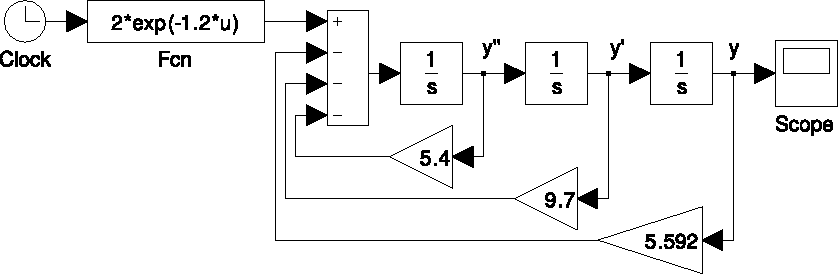
\includegraphics{misc/Obr_SimSchema_FontPokus.pdf}
    }

    \caption{Simulačná schéma}
	\label{Simulačná schéma}
\end{figure}




\begin{figure}[!ht]
	\centering

    \makebox[\textwidth][c]{%
	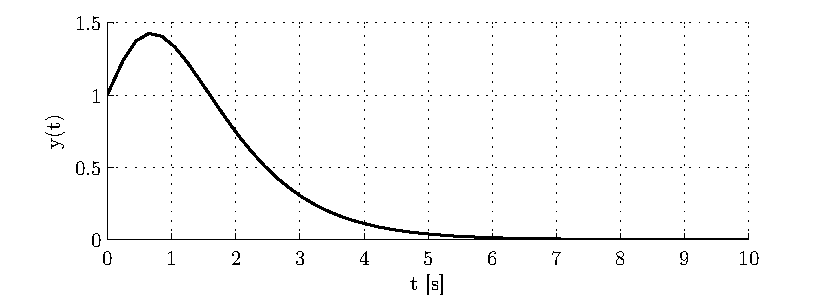
\includegraphics{misc/Obr_Simulink.pdf}
    }

    \caption{Simuláciou získaný časový priebeh}
	\label{Simuláciou získaný časový priebeh}
\end{figure}









\section{Analyticky}



Rovnica \eqref{Zadaná rovnica} je nehomogénna lineárna diferenciálna rovnica s konštantnými koeficientami tretieho rádu ($n_r = 3$). Jej Charakteristická rovnica je
\begin{equation}
	s^3 + 5,4 s^2 + 9,7 s + 5,592 = 0
\end{equation}
Riešeniami Charakteristickej rovnice sú
\begin{equation} \label{Korene CHR}
		s_1 = -2,1 + 0,5i \qquad
		s_2 = -2,1 - 0,5i \qquad
		s_3 = -1,2
\end{equation}
Fundamentálne riešenia (módy) rovnice \eqref{Zadaná rovnica} zodpovedajúce jednotlivým riešeniam Charakteristickej rovnice sú
\begin{subequations}
	\begin{align}
		y_1(t) &= e^{(-2,1 + 0,5i)t} = e^{-2,1t} \big({ \cos(0,5t) + i\sin(0.5t) }\big) \\
		y_2(t) &= e^{(-2,1 - 0,5i)t} = e^{-2,1t} \big({ \cos(0,5t) - i\sin(0.5t) }\big) \\
		y_3(t) &= e^{-1.2t}
	\end{align}
\end{subequations}




% \noindent
% \hrule
%
% \medskip

% \noindent



Totiž, vo všeobecnosti možno rozlišovať niekoľko prípadov, pre ktoré platí:
\begin{enumerate}
    \item Ak má charakteristická rovnica $n$ navzájom rôznych riešení $s_i$ pre $i = 1, \ldots, n$, potom zodpovedajúce fundamentálne riešenia (módy) sú: $e^{s_1 t}$, $e^{s_2 t}$, \ldots, $e^{s_n t}$.
    \item Ak sa medzi $n$ koreňmi charakteristického polynómu vyskytne $k$-násobný koreň, vytvoríme $k$ lineárne závislých riešení: $e^{s_i t}$, $t e^{s_i t}$, \ldots, $t^{k-1} e^{s_i t}$
    \item V prípade výskytu dvojice komplexne združených koreňov charakteristického polynómu, $s_{1,2} = \alpha \pm j \beta$, kde $j$ je imaginárna jednotka, využijeme na určenie fundamentálnych riešení Eulerov vzťah
    \begin{equation}
        e^{\left(\alpha \pm j \beta\right)t} = e^{\alpha t} \left( \cos\beta t \pm j \sin \beta t\right)
    \end{equation}
    Preto potom možno písať príslušné fundamentálne riešenie v tvare
    \begin{equation}
        c_1 e^{\left(\alpha + j \beta\right)t} + c_2 e^{\left(\alpha - j \beta\right)t} = e^{\alpha t} \left( c^\prime \cos\beta t + c^{\prime\prime} \sin \beta t\right)
    \end{equation}
    kde sú imaginárne časti nulové.
\end{enumerate}



% \noindent
% \hrule
%
% \bigskip




Výsledné reálne všeobecné riešenie homogénnej časti má tvar
\begin{equation} \label{Výsledné reálne všeobecné riešenie homogénnej}
	y_{h_{vs}}(t) = c_1 e^{-2,1t} \cos(0,5t) + c_2 e^{-2,1t} \sin(0,5t) + c_3 e^{-1.2t}
\end{equation}
kde $c_1$, $c_2$ a $c_3$ sú reálne konštanty.




Pravá strana $q(t)$ diferenciálnej rovnice \eqref{Zadaná rovnica} má vo všeobecnosti tvar $q(t) = e^{\alpha t} P_n(t)$, pričom platí
\begin{subequations}
	\begin{align}
		P_n(t) &= 2 \\
		\alpha &= -1,2
	\end{align}
\end{subequations}
Pre tento špeciálny tvar pravej strany má partikulárne riešenie $\psi(t)$ tvar $\psi(t) = t^k e^{\alpha t} Q_n(t)$, kde $k$ je násobnosť koreňa $\alpha$ a $Q_n(t)$ je všeobecný polynóm rovnakého stupňa ako $P_n(t)$. V tomto prípade
\begin{subequations}
	\begin{align}
		k &= 1 \\
		Q_n(t) &= A_0
	\end{align}
\end{subequations}
Partikulárne riešenie $\psi(t)$ určíme použitím metódy neurčitých koeficientov, a teda partikulárne riešenie a jeho derivácie dosadíme do diferenciálnej rovnice.
\begin{subequations} \label{derivacieParRies}
	\begin{align}
		\psi(t) &= A_0 t e^{-1,2 t} \\
		\dot{\psi}(t) &=  A_0 e^{-1,2t} - 1,2 A_0 t e^{-1,2t}\\
		\ddot{\psi}(t) &= -2,4 A_0 e^{-1,2t} + 1,44 A_0 t e^{-1,2t} \\
		\dddot{\psi}(t) &= 4,32 A_0 e^{-1,2t} - 1,728 A_0 t e^{-1,2t}
	\end{align}
\end{subequations}
Rovnice \eqref{derivacieParRies} dosadíme do diferenciálnej rovnice \eqref{Zadaná rovnica} a upravíme.
\begin{subequations}
\begin{align}
	\begin{split}
		2 e^{-1,2t} &=
		 4,32 A_0 e^{-1,2t} - 1,728 A_0 t e^{-1,2t}  + 5,4 \left( -2,4 A_0 e^{-1,2t} + 1,44 A_0 t e^{-1,2t} \right) \\
		& + 9,7  \left( A_0 e^{-1,2t} - 1,2 A_0 t e^{-1,2t} \right) + 5,592 \left( A_0 t e^{-1,2 t} \right)
	\end{split} \\
	\begin{split}
		2 e^{-1,2t} &=
		 4,32 A_0 e^{-1,2t} - 1,728 A_0 t e^{-1,2t} - 12,96 A_0 e^{-1.2t} + 7,776 A_0 t e^{-1,2t}  \\
		& + 9,7  A_0 e^{-1,2t} - 8,5 A_0 t e^{-1,2t} + 5,592  A_0 t e^{-1,2 t}
	\end{split} \\
	\begin{split} \label{dosadenePartikRies}
		2 e^{-1,2t} &=
		 1,06 A_0 e^{-1,2t} + 3,14 t e^{-1,2 t}
	\end{split}
\end{align}
\end{subequations}
Z \eqref{dosadenePartikRies} vyplýva
\begin{equation}
	2 = 1,06 A_0 \qquad \Rightarrow \qquad A_0 = \frac{2}{1,06} \doteq 1,8868
\end{equation}
a partikulárne riešenie $\psi(t)$ je
\begin{equation} \label{Partikulárne riešenie}
	\psi(t) = 1,8868 t e^{-1,2 t}
\end{equation}







Všeobecné riešenie diferenciálnej rovnice \eqref{Zadaná rovnica} je súčet \eqref{Výsledné reálne všeobecné riešenie homogénnej} s \eqref{Partikulárne riešenie}:
\begin{subequations}
\begin{equation} \label{Všeobecné riešenie}
	y_{vs}(t) = c_1 e^{-2,1t} \cos(0,5t) + c_2 e^{-2,1t} \sin(0,5t) + c_3 e^{-1.2t} + 1,8868 t e^{-1,2 t}
\end{equation}
Konštanty $c_1$, $c_2$ a $c_3$ sú dané konkrétnymi začiatočnými podmienkami, ktoré sa dosadia do príslušných derivácií všeobecného riešenia. V tomto prípade sú potrebné okrem nultej derivácie \eqref{Všeobecné riešenie} aj prvá a druhá derivácia všeobecného riešenia:
\begin{align}
	\begin{split} \label{prvaDer Všeobecné riešenie}
		\dot y_{vs}(t) &= 1,8868e^{-1,2 t}  -2,2642te^{-1,2 t} - 1,2 c_3 e^{-1,2t} - 2,1 c_2 e^{-2,1t} \sin(0,5t) \\&+ 0,5 c_2 e^{-2,1t} \cos(0,5t) - 2,1 c_1 e^{-2,1t} \cos(0,5t) - 0,5 c_1 e^{-2,1t} \sin(0,5t)
	\end{split} \\
	\begin{split} \label{druhaDer Všeobecné riešenie}
		\ddot y_{vs}(t) &= -4,5283 e^{-1.2t} + 2,717 t e^{-1.2t} + 1,44 c_3 e^{-1.2t} + 4,16 c_2 e^{-2.1t} \sin(0.5t) \\&- 2.1 c_2 e^{-2.1t} \cos(0.5t) + 4,16 c_1 e^{-2.1t} \cos(0.5t) + 2.1 c_1 e^{-2.1t} \sin(0.5t)
	\end{split}
\end{align}
\end{subequations}










Dosadením začiatočných podmienok do \eqref{Všeobecné riešenie}, \eqref{prvaDer Všeobecné riešenie} a \eqref{druhaDer Všeobecné riešenie} získame sústavu troch rovníc o troch neznámych, ktorá má v maticovom zápise tvar
\begin{equation}
	\begin{bmatrix}
		   1 &    0 &    1 \\
		-2,1 &  0,5 & -1,2 \\
		4,16 & -2,1 & 1,44
	\end{bmatrix}
	\begin{bmatrix}
		c_1 \\
		c_2 \\
		c_3
	\end{bmatrix}
	=
	\begin{bmatrix}
		1 \\
		1-1,8868 \\
		1+4,5283
	\end{bmatrix}
\end{equation}
a jej riešením je
\begin{subequations}
	\begin{align}
		c_1 &= -5,0979\\
		c_2 &= -8,5498\\
		c_3 &=  6,0979
	\end{align}
\end{subequations}




Riešením diferenciálnej rovnice \eqref{Zadaná rovnica} je
\begin{equation}
	y(t) = -5,0979 e^{-2,1t} \cos(0,5t)  -8,5498 e^{-2,1t} \sin(0,5t) + 6,0979 e^{-1.2t} + 1,8868 t e^{-1,2 t}
\end{equation}
Graficky je riešenie znázornené na Obr. \ref{Grafické znázornenie riešenia získaného analyticky}.


\begin{figure}[!ht]
	\centering

    \makebox[\textwidth][c]{%
	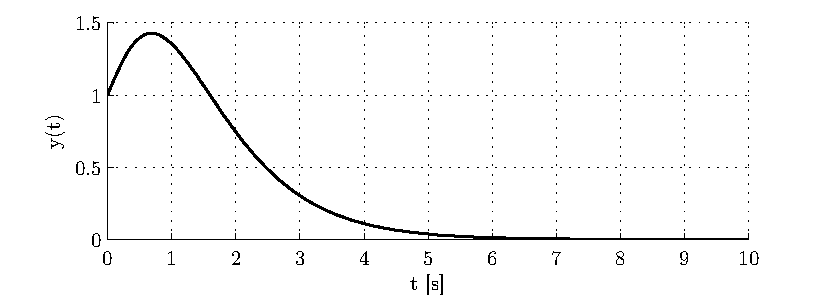
\includegraphics{misc/Obr_GrafRucne.pdf}
    }

	\caption{Grafické znázornenie riešenia získaného analyticky}
	\label{Grafické znázornenie riešenia získaného analyticky}
\end{figure}














\section{Pomocou Laplaceovej transformácie}



Rovnica \eqref{Zadaná rovnica} má po Laplaceovej transformácii tvar
\begin{equation}
	s^3Y - s^2 - s - 1 + 5,4 \left( s^2Y - s - 1 \right) + 9,7 \left( sY - 1 \right) + 5,592 Y = \frac{2}{\left( s+1,2 \right)}
\end{equation}
Po úprave
\begin{subequations}
	\begin{align}
		& s^3Y - s^2 - s - 1 + 5,4s^2Y - 5,4s - 5,4 + 9,7sY - 9,7 + 5,592 Y = \frac{2}{\left( s+1,2 \right)} \\
		& Y \left( s^3 + 5,4s^2 + 9,7s + 5,592 \right) + \left( - s^2 - s - 1 - 5,4s - 5,4 - 9,7  \right) = \frac{2}{\left( s+1,2 \right)} \\
		& Y \left( s^3 + 5,4s^2 + 9,7s + 5,592 \right) + \left( - s^2 - 6,4s - 16,1 \right) = \frac{2}{\left( s+1,2 \right)} \\
		& Y = \frac{2}{\left( s+1,2 \right) \left( s^3 + 5,4s^2 + 9,7s + 5,592 \right)} + \frac{\left(  s^2 + 6,4s + 16,1 \right)}{ \left( s^3 + 5,4s^2 + 9,7s + 5,592 \right)} \label{ZlaplasovaneNeupravene}
	\end{align}
\end{subequations}
Korene polynómu $s^3 + 5,4s^2 + 9,7s + 5,592$ sú \eqref{Korene CHR} a korene polynómu $s^2 + 6,4s + 16,1$ sú
\begin{equation} \label{Korene citatela vlastnejZ}
		s_4 = -3,2 + 2,4207i \qquad
		s_5 = -3,2 - 2,4207i
\end{equation}
a teda \eqref{ZlaplasovaneNeupravene} je možné napísať v tvare
\begin{equation}
	\begin{split}
		Y &= \frac{2}{\left( s+2,1-0,5i \right)\left( s+2,1+0,5i \right)\left( s+1,2 \right)^2 } \\&+ \frac{\left(  s +3,2 - 2,4207i \right)\left(  s +3,2 + 2,4207i \right)}{ \left( s+2,1-0,5i \right)\left( s+2,1+0,5i \right)\left( s+1,2 \right)} \\
		 & = Y_1 + Y_2
	\end{split}
\end{equation}






Na spätnú Laplaceovu transformáciu využijeme Heavisideov rozvojový vzorec
\begin{equation} \label{Heavisideov rozvojový vzorec}
	y(t) = \sum_{i=1}^k e^{s_i t} \sum_{j=1}^{r_i} \frac{\left[ G_i^{(r_i-j)} (s) \right]_{s = s_i}}{(r_i - j)!(j - 1)!}t^{j-1}
\end{equation}
kde $G_i = Y(s) \left( s - s_i \right)^{r_i}$, $s_i \  (i = 1, \ldots, j)$ sú póly prenosovej funkcie $Y(s)$ a $r_i \  (i = 1, \ldots, j)$ je ich násobnosť.



\paragraph{Spätná transformácia $Y_1(s)$.}
Najprv je potrebné určiť hodnoty $\left[ G_i^{(r_i-j)} (s) \right]_{s = s_i}$:
\begin{subequations}
	\begin{align}
		G_1(s_1) &= \frac{2}{\left( -2,1 + 0,5i+2,1+0,5i \right)\left( -2,1 + 0,5i+1,2 \right)^2 } = 1,602 - 0,9968i \\
		G_2(s_2) &= \frac{2}{\left( -2,1 + 0,5i+2,1-0,5i \right)\left( -2,1 + 0,5i+1,2 \right)^2 } = 1,602 + 0,9968i \\
		G_3(s_3) &= \frac{2}{\left( -1,2+2,1-0,5i \right)\left( -1,2+2,1+0,5i \right)} = 1.8868 \\
		\dot{G}_3(s_3) &= - \frac{2\left( 2s_3 + 4,2 \right)}{\left( s_3^2 +4,2s_3 +4.66 \right)^2} = - \frac{2\left( 2(-1,2) + 4,2 \right)}{\left( (-1,2)^2 +4,2(-1,2) +4.66 \right)^2} = -3.204
	\end{align}
\end{subequations}
Tieto hodnoty sa potom dosadia do \eqref{Heavisideov rozvojový vzorec} a po úprave:
\begin{subequations}
	\begin{align}
		\begin{split}
			y_1(t) &= e^{(-2,1 + 0,5i)t}\left( 1,602 - 0,9968i \right) + e^{(-2,1 - 0,5i)t}\left( 1,602 + 0,9968i \right) \\
			       &+ e^{-1,2t}\left( \frac{-3,204}{(2-1)!(1-1)!}t^0 + \frac{1,8868}{(2-2)!(2-1)!}t^1\right)
		\end{split}	\\
		\begin{split}
			y_1(t) &= e^{-2,1t} \left( 3,204 \cos(0,5t) +1,9936 \sin(0,5t) \right) -3,204 e^{-1,2t} + 1,8868te^{-1,2t}
		\end{split}
	\end{align}
\end{subequations}



\paragraph{Spätná transformácia $Y_2(s)$:}
Určenie hodnôt $\left[ G_i^{(r_i-j)} (s) \right]_{s = s_i}$ pre prípad $Y_2(s)$:
\begin{subequations}
	\begin{align}
        \begin{split}
		G_1(s_1) &= \frac{\left( -2,1 + 0,5i + 3,2 - 2,4207i \right)\left( -2,1 + 0,5i + 3,2 + 2,4207i \right)}
		                 {\left( -2,1 + 0,5i + 2,1 + 0,5i \right)\left( -2,1 + 0,5i + 1,2 \right) }
		                 \\&= -4,1508 + 5,2715i
        \end{split}\\
        \begin{split}
		G_2(s_2) &= \frac{\left( -2,1 - 0,5i + 3,2 - 2,4207i \right)\left( -2,1 - 0,5i + 3,2 + 2,4207i \right)}
		                 {\left( -2,1 - 0,5i + 2,1 - 0,5i \right)\left( -2,1 - 0,5i + 1,2 \right) }
		                 \\&= -4,1508 - 5,2715i
        \end{split}\\
		G_3(s_3) &= \frac{\left( -1,2 + 3,2 - 2,4207i \right)\left( -1,2 + 3,2 + 2,4207i \right)}
		                 {\left( -1,2 + 2,1 - 0,5i \right)\left( -1,2 + 2,1 + 0,5i \right) }
		                 = 9,3017
	\end{align}
\end{subequations}
A potom:
\begin{subequations}
	\begin{align}
		\begin{split}
			y_2(t) &= e^{(-2,1 + 0,5i)t}\left( -4,1508 + 5,2715i \right) \\&+ e^{(-2,1 - 0,5i)t}\left( -4,1508 - 5,2715i \right) + 9,3017 e^{-1,2t}
		\end{split}	\\
		\begin{split}
			y_2(t) &= e^{-2,1t} \left( -8,3016 \cos(0,5t) -10,543 \sin(0,5t) \right) + 9,3017 e^{-1,2t}
		\end{split}
	\end{align}
\end{subequations}




Výsledné riešenie je súčtom $y_1(t)$ s $y_2(t)$
\begin{equation}
	\begin{split}
		y(t) &= y_1(t) + y_2(t) = e^{-2,1t} \left( -5,0976 \cos(0,5t) -8,5494 \sin(0,5t) \right) \\&+6,0977 e^{-1,2t} + 1,8868te^{-1,2t}
	\end{split}
\end{equation}
Grafické znázornenie riešenia je na Obr. \ref{Grafické znázornenie riešenia získaného pomocou Laplaceovej transformácie}.

\begin{figure}[!ht]
	\centering

    \makebox[\textwidth][c]{%
	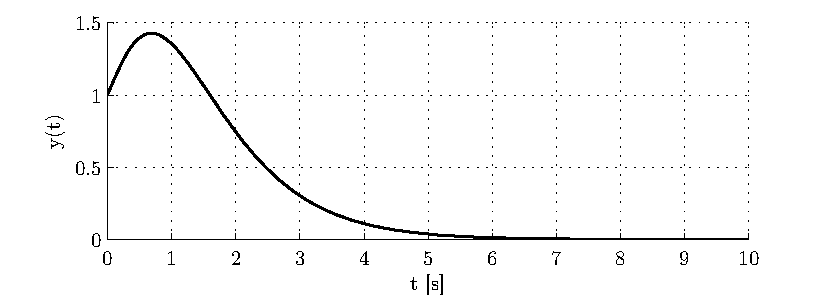
\includegraphics{misc/Obr_Laplaceovou.pdf}
    }

	\caption{Grafické znázornenie riešenia získaného pomocou Laplaceovej transformácie}
	\label{Grafické znázornenie riešenia získaného pomocou Laplaceovej transformácie}
\end{figure}














\section{Pomocou Symbolic toolboxu (MATLAB)}



Pre výpočet riešenia pomocou toolboxu Symbolic je potrebné zadať nasledujúce príkazy:
\begin{lstlisting}[language=Matlab,]
yt = dsolve('D3y + 5.4*D2y + 9.7*Dy + 5.592*y = 2*exp(-1.2*t)','y(0)=1','Dy(0)=1','D2y(0)=1')

ezplot(yt,[0 10])
\end{lstlisting}
Odpoveďou je riešenie a vykreslenie jeho priebehu znázornené na Obr. \ref{Grafické znázornenie riešenia získaného Symbolic}.
{\footnotesize
\begin{verbatim}
yt =

100/53*t*exp(-6/5*t)+17129/2809*exp(-6/5*t)-120082/14045*exp(-21/10*t)*sin(1/2*t)
-14320/2809*exp(-21/10*t)*cos(1/2*t)
\end{verbatim}}


\begin{figure}[!ht]
	\centering

    \makebox[\textwidth][c]{%
	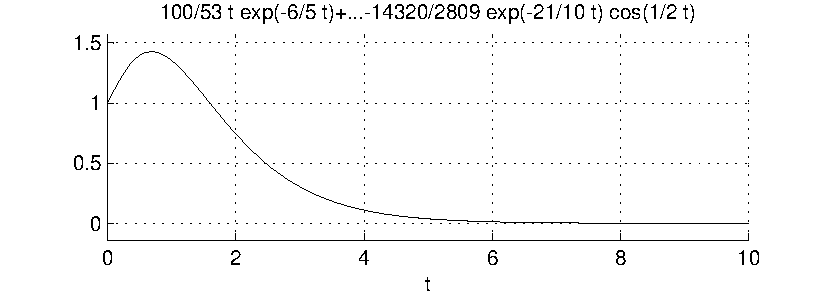
\includegraphics{misc/Obr_Symbolic.pdf}
    }

	\caption{Grafické znázornenie riešenia získaného pomocou toolboxu Symbolic}
	\label{Grafické znázornenie riešenia získaného Symbolic}
\end{figure}































\section{Pomocou ODE solvera -- numerické riešenie (MATLAB)}


Pre numerický výpočet riešenia pomocou procedúry \verb|ode45| je potrebné previesť diferenciálnu rovnicu \eqref{Zadaná rovnica} na systém diferenciálnych rovníc 1. rádu. V tomto prípade:
\begin{subequations}
	\begin{align}
		\dot x_1 &= x_2 \\
		\dot x_2 &= x_3 \\
		\dot x_3 &= -5,4 x_3 -9,7 x_2 -5,592 x_1 + 2 e^{-1,2 t}
	\end{align}
\end{subequations}
Tento systém sa potom zapíše ako funkcia, ktorú bude procedúra \verb|ode45| používať
\begin{lstlisting}[language=Matlab,]
function dx = fundif(t,x);
dx(1) = x(2);
dx(2) = x(3);
dx(3) = -5.4*x(3) -9.7*x(2) -5.592*x(1) + 2*exp(-1.2*t);
dx = dx(:);
\end{lstlisting}

Samotné použitie procedúry \verb|ode45| sa vykoná nasledovnými príkazmi:
\begin{lstlisting}[language=Matlab,]
[t,y] = ode45('fundif',[0 10],[1; 1; 1]);
plot(t,y(:,1))
\end{lstlisting}
Výsledný priebeh riešenia je na Obr. \ref{Grafické znázornenie riešenia získaného pomocou ode45}.
\begin{figure}[!ht]
	\centering

    \makebox[\textwidth][c]{%
	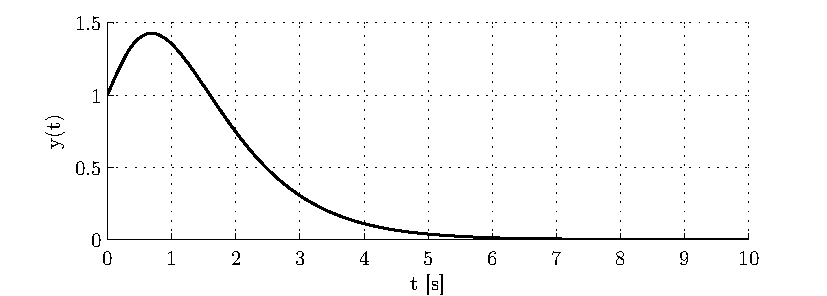
\includegraphics{misc/Obr_ode45.pdf}
    }

    \caption{Grafické znázornenie riešenia získaného pomocou ode45}
	\label{Grafické znázornenie riešenia získaného pomocou ode45}
\end{figure}











\end{document}
